We demonstrate the accuracy and efficiency of the ISDF-CVT method for hybrid
functional calculations by using the DGDFT (Discontinuous Galerkin Density
Functional Theory) software package \cite{JCP_231_2140_2012_DGDFT,
JCP_143_124110_2015_DGDFT,PCCP_17_31397_2015_DGDFT, JCP_145_154101_2016_DGDFT,
JCP_335_426_2017_DGDFT}. DGDFT is a massively parallel electronic structure
software package designed for large scale DFT calculations involving up to tens
of thousands of atoms. It includes a self-contained module called PWDFT for
performing planewave based electronic structure calculations (mostly for
benchmark and validation purposes). We implemented the ISDF-CVT method in PWDFT.
We use the Message Passing Interface (MPI) to handle data communication. We use
the Hartwigsen-Goedecker-Hutter (HGH) norm-conserving pseudopotential
\cite{PRB_58_3641_1998_HGH}. The atomic valence electron configuration is 1s$^1$
for the H atom, 2s$^2$2p$^1$ for the B atom, 2s$^2$2p$^3$ for the N atom,
2s$^2$2p$^4$ for the O atom, 3s$^2$3p$^2$ for the Si atom in our DFT
calculations, respectively. All calculations use the HSE06 functional 
\cite{JCP_124_219906_2006_HSE06}, carried out on the Edison systems at the
National Energy Research Scientific Computing Center (NERSC). Each node consists
of two Intel ``Ivy Bridge'' processors with 24 cores in total and 64 gigabyte 
(GB) of memory. Our implementation only uses MPI. The number of cores is equal
to the number of MPI ranks used in the simulation.


In this section, we demonstrate the performance of the ISDF-CVT method for
accelerating hybrid functional calculations by using three types of systems 
\cite{JCTC_2017_PCDIIS}. They consist of bulk silicon systems (Si$_{64}$, Si$_
{216}$, and Si$_{1000}$), a bulk water system with $64$ molecules ((H$_2$O)$_
{64}$), and a disordered silicon aluminum alloy system (Al$_{176}$Si$_{24}$).
Bulk silicon systems (Si$_{64}$, Si$_{216}$ and Si$_{1000}$) and bulk water
system ((H$_2$O)$_{64}$) are semiconducting with a relatively large energy gap
$E_\text{gap} > 1.0$ eV, and the Al$_{176}$Si$_{24}$ system is metallic with a
small energy gap $E_\text{gap} < 0.1$ eV. All systems are closed shell systems,
and the number of occupied bands is $N_\text{band} = N_{e}/2$, where $N_e$ is
the number of valence electrons. In order to compute the energy gap in the
systems, we also include two unoccupied bands in all calculations.


\subsection{\numintitle{Accuracy: Si$_{216}$ and Al$_{176}$Si$_{24}$}}
\label{c5subsec:accuracy}

We demonstrate the accuracy of the CVT-based ISDF decomposition in the hybrid
functional calculation for semiconducting Si$_{216}$ and metallic Al$_{176}$Si$_
{24}$ systems, respectively. Although there is no general theoretical guarantee
for the convergence of the K-Means algorithm and the convergence can depend
sensitively on the initialization \cite{arthur2006slow,arthur2007k}, we find
that, in the current context,  initialization to have little impact on the final
accuracy of the approximation. Hence we use random initialization for the
K-Means algorithm. In all calculations, the adaptively compressed exchange (ACE)
technique is used to accelerate hybrid functional calculations without loss of
accuracy \cite{JCTC_12_2242_2016_ACE}. The results obtained in this work are
labeled as ACE-ISDF (CVT), which are compared against those obtained from the
previous work based on the QRCP decomposition \cite{JCTC_2017_ISDF} labeled as
ACE-ISDF (QRCP). In both cases, we introduce a rank parameter $c$ to control the
trade-off between efficiency and accuracy, by setting the number of
interpolation points $N_\mu = cN_e$. We measure the error using the valence band
maximum (VBM) energy level, the conduction band minimum (CBM) energy level, the
energy gap, the Hartree-Fock exchange energy, the total energy, and the atomic
forces, respectively. We remark that, in ISDF-CVT and ISDF-QRCP, the atomic
force is computed directly using the Hellmann-Feynman formula, thereby neglects
the Pulay force contribution from the change of the interpolation points. On the
other hand, there is no Pulay contribution in the ACE formulation, and the
Hellmann-Feynman force $F_I^\text{ACE}$ can be used as the reference solution.

The last three quantities are defined as
\begin{align*}
	\Delta{E_\text{HF}} &= \abs{E_\text{HF}^\text{ACE-ISDF (CVT)} - E_\text{HF}^
	\text{ACE}}/N_{A}\\
	\Delta{E} &= \abs{E^\text{ACE-ISDF (CVT)} - E^\text{ACE}}/N_{A}\\
	{\Delta}F &= \max_I\norm{F_I^\text{ACE-ISDF (CVT)} - F_I^\text{ACE}}
\end{align*}
where $N_A$ is the number of atoms and $I$ is the atom index.

Table~\ref{tab:Accuracy} shows that the accuracy of the ACE-ISDF (CVT) method
can systematically improve as the rank parameter $c$ increases. When the rank
parameter is large enough ($\mathbin{\Geq}20.0$), the results from ACE-ISDF 
(CVT) are fully comparable (the energy error is below $10^{-6}\HaPA$ and the
force error is below $10^{-5}\HaPB$) to those obtained from the benchmark
calculations. Furthermore, for a moderate choice of the rank parameter $c=6.0$,
the error of the energy per atom reaches below the chemical accuracy of 1
kcal/mol ($1.6\times 10^{-3}\HaPA$), and the error of the force is around $10^
{-3}\HaPB$. This is comparable to the accuracy obtained from ACE-ISDF (QRCP),
and to e.g. linear scaling methods for insulating systems with reasonable amount
of truncation needed to achieve significant speedup \cite{JCTC_11_4655_2015}. In
fact, when compared with ACE-ISDF (QRCP) in Figure~\ref{fig:Si216Al176Si24}, we
find that the CVT based ISDF decomposition achieves slightly higher accuracy,
though there is no theoretical guarantee for this to hold in general. The last
column of Table~\ref{tab:Accuracy} shows the runtime of the K-Means algorithm.
As $c$ increases, the number of interpolation points as well as the number of
cells increases proportionally. Hence we observe that the runtime of K-Means
scales linearly with respect to $c$.

\begin{table}[htbp]
	\centering
	\caption{Accuracy of ACE-ISDF Based Hybrid Functional Calculations 
	(HSE06) Obtained by Using the CVT method To Select Interpolation Points,
	with Varying Rank Parameter $c$ for Semiconducting Si$_{216}$ and Metallic
	Al$_{176}$Si$_{24}$ Systems\textsuperscript{$\alpha$}.}\label{tab:Accuracy}
	\begin{threeparttable}
		\begin{tabular}{cccccccc}
			\rowcolor{lightgray}$c$  &  $E_\text{VBM}$ & $E_\text{CBM}$ & $E_\text{gap}$
			& ${\Delta}E_\text{HF}$ & ${\Delta}E$ & ${\Delta}F$ & T\textsubscript{KMEANS} \\
			\multicolumn{8}{c}{\multirow{2}{*}{ACE-ISDF: Semiconducting Si$_{216}$ ($N_\text{band}=432$)}} \\ \\
			 4.0 & 6.7467 & 8.3433 & -1.5967 &  2.69E-03 &  3.08E-03 &  5.04E-03 &  0.228 \ \\
			 5.0 & 6.6852 & 8.2231 & -1.5379 &  9.46E-04 &  1.12E-03 &  2.29E-03 &  0.248 \ \\
			 6.0 & 6.6640 & 8.1522 & -1.4882 &  3.76E-04 &  4.62E-04 &  1.05E-03 &  0.301 \ \\
			 7.0 & 6.6550 & 8.1163 & -1.4613 &  1.55E-04 &  1.98E-04 &  6.49E-04 &  0.312 \ \\
			 8.0 & 6.6510 & 8.1030 & -1.4520 &  7.33E-05 &  9.55E-05 &  3.07E-04 &  0.349 \ \\
			 9.0 & 6.6490 & 8.0980 & -1.4490 &  3.60E-05 &  4.96E-05 &  2.30E-04 &  0.398 \ \\
			10.0 & 6.6479 & 8.0959 & -1.4480 &  1.78E-05 &  2.64E-05 &  1.30E-04 &  0.477 \ \\
			12.0 & 6.6472 & 8.0945 & -1.4473 &  4.46E-06 &  8.91E-06 &  8.37E-05 &  0.530 \ \\
			16.0 & 6.6469 & 8.0937 & -1.4468 &  1.51E-07 &  1.41E-06 &  3.20E-05 &  0.773 \ \\
			20.0 & 6.6468 & 8.0935 & -1.4467 &  4.06E-07 &  3.33E-07 &  1.20E-05 &  0.830 \ \\
			24.0 & 6.6468 & 8.0935 & -1.4467 &  2.99E-07 &  1.06E-07 &  5.18E-06 &  0.931 \ \\
			 ACE & 6.6468 & 8.0934 & -1.4466 &  0.00E+00 &  0.00E+00 &  0.00E+00 &  - \ \\
			\multicolumn{8}{c}{\multirow{2}{*}{ACE-ISDF: Metallic Al$_{176}$Si$_{24}$ ($N_\text{band} =312$)}} \\ \\
			 4.0 & 7.9258 & 8.0335 & -0.1076 &  3.80E-03 &  4.03E-03 &  8.01E-03 &  0.430 \ \\
			 5.0 & 7.8537 & 7.9596 & -0.1059 &  1.60E-03 &  1.69E-03 &  3.18E-03 &  0.535 \ \\
			 6.0 & 7.8071 & 7.9127 & -0.1056 &  6.07E-04 &  6.39E-04 &  1.48E-03 &  0.611 \ \\
			 7.0 & 7.7843 & 7.8860 & -0.1017 &  2.07E-04 &  2.17E-04 &  1.03E-03 &  0.731 \ \\
			 8.0 & 7.7749 & 7.8749 & -0.1000 &  7.43E-05 &  7.77E-05 &  4.40E-04 &  0.948 \ \\
			 9.0 & 7.7718 & 7.8710 & -0.0992 &  3.02E-05 &  3.20E-05 &  1.98E-04 &  0.947 \ \\
			10.0 & 7.7709 & 7.8697 & -0.0989 &  1.48E-05 &  1.60E-05 &  1.80E-04 &  1.096 \ \\
			12.0 & 7.7703 & 7.8690 & -0.0987 &  4.64E-06 &  5.60E-06 &  8.51E-05 &  1.305 \ \\
			16.0 & 7.7702 & 7.8688 & -0.0986 &  6.35E-07 &  1.41E-06 &  3.24E-05 &  1.646 \ \\
			20.0 & 7.7701 & 7.8687 & -0.0986 &  1.70E-08 &  5.30E-07 &  1.91E-05 &  2.037 \ \\
			 ACE & 7.7701 & 7.8687 & -0.0986 &  0.00E+00 &  0.00E+00 &  0.00E+00 &  - \ \\
		\end{tabular}
		\begin{tablenotes}
			\item[$\alpha$] The unit for VBM ($E_\text{VBM}$), CBM ($E_\text{CBM}$)
			and the energy gap $E_\text{gap}$ is eV. The unit for the error in the
			Hartree-Fock exchange energy ${\Delta}E_\text{HF}$ and the total energy
			${\Delta}E$ is Ha/atom, and the unit for the error in atomic forces 
			${\Delta}F$ is Ha/Bohr. We use the results from the ACE-enabled hybrid
			functional calculations as the reference. The last column shows the time 
			(in seconds) for K-Means with different $c$ values, with 434 cores for
			Si$_{216}$ and 314 cores for Al$_{176}$Si$_{24}$ on Edison.
		\end{tablenotes}
	\end{threeparttable}
\end{table}

\begin{figure}[htbp]
	\begin{center}
		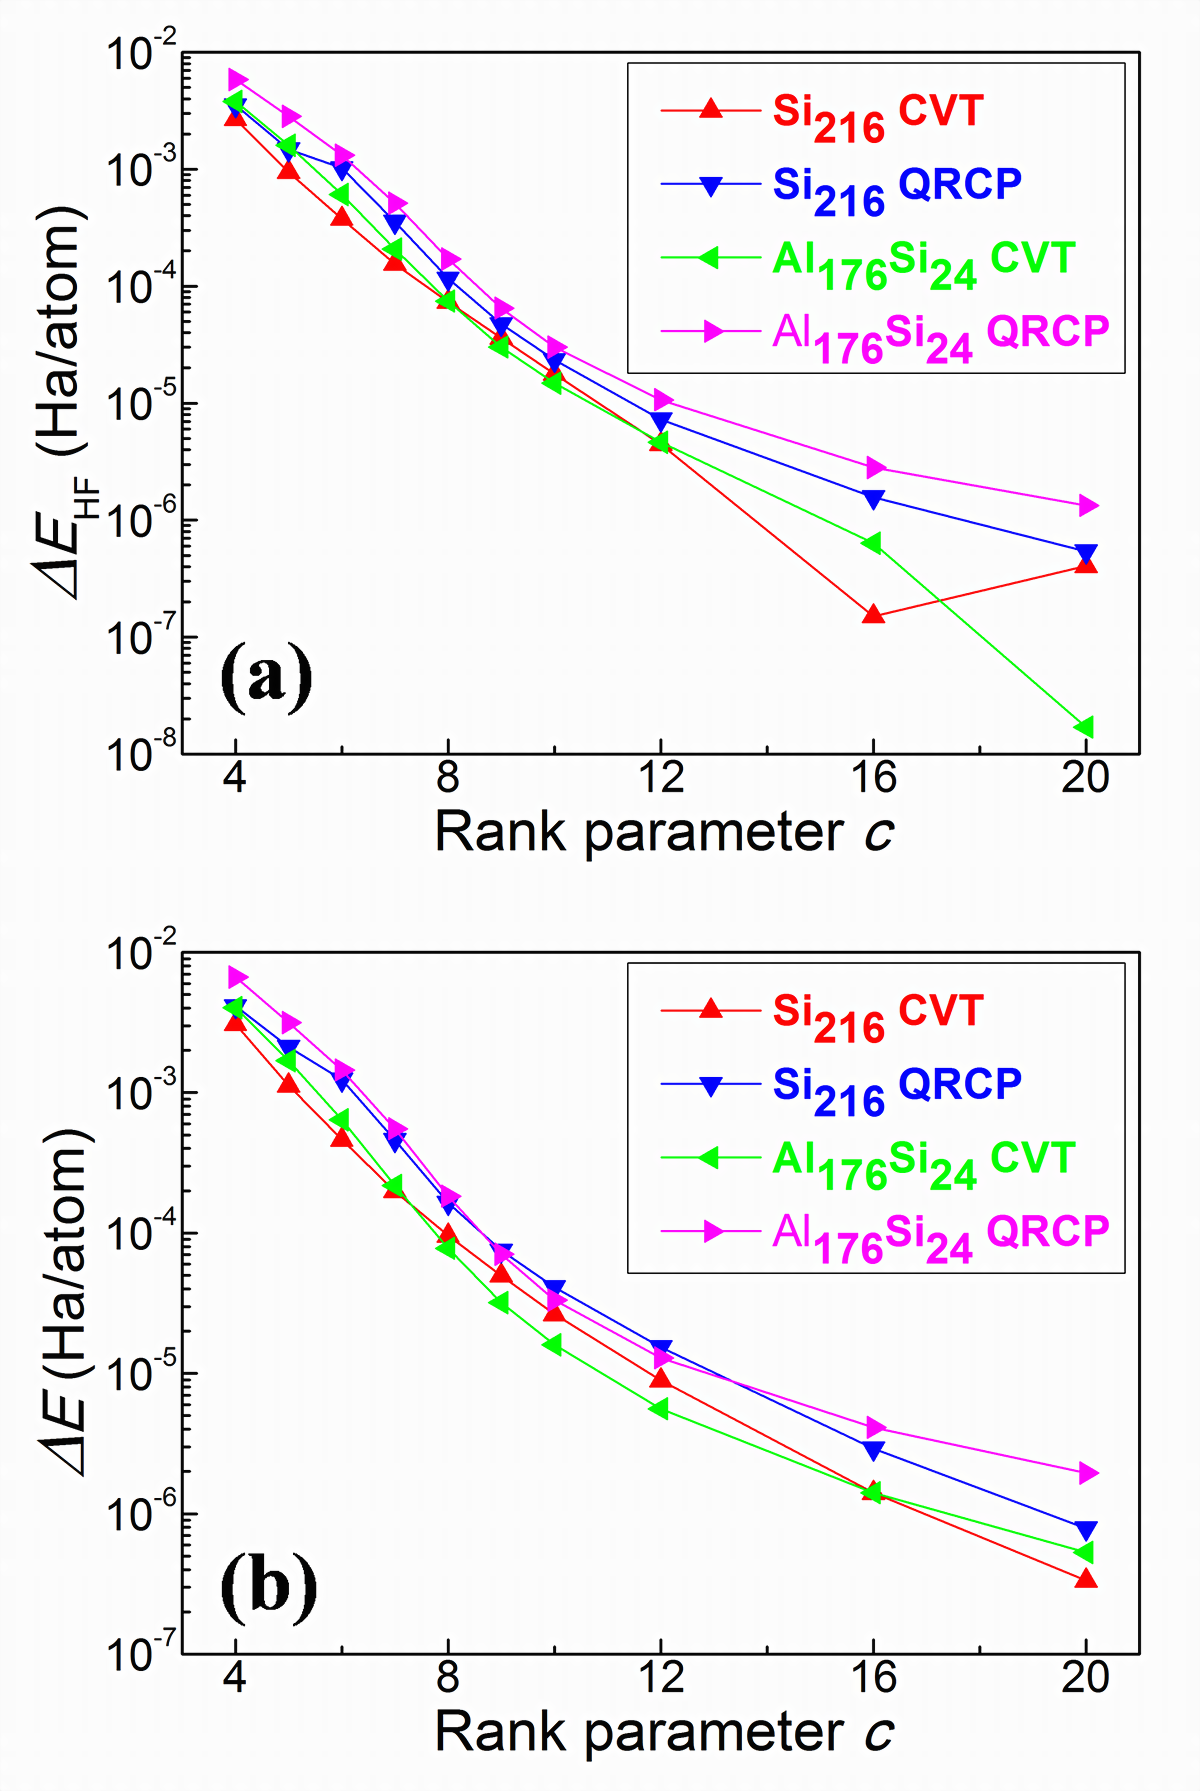
\includegraphics[width=0.8\textwidth]{./cvt/pics/Si216Al176Si24.pdf}
	\end{center}
	\caption{The accuracy of ACE-ISDF based hybrid functional calculations (HSE06)
	obtained by using the CVT and QRCP procedures to select the interpolation
	points, with varying rank parameter $c$ from 4 to 20 for Si$_{216}$ and Al$_
	{176}$Si$_{24}$, including the error of (a) Hartree-Fock exchange energy $
	{\Delta}E_\text{HF}$ (Ha/atom) and (b) total energy ${\Delta}E$ (Ha/atom).} 
	\label{fig:Si216Al176Si24}
\end{figure}

\subsection{\numintitle{Efficiency: Si$_{1000}$}}\label{c5subsec:si1000}

We report the efficiency of the ISDF-CVT method by performing hybrid DFT
calculations for a bulk silicon system with 1000 atoms ($N_\text{band} \Eq
2000$) on 2000 computational cores as shown in Table~\ref{tab:Efficiency}, with
respect to various choices of the kinetic energy cutoff ($E_{\text{cut}}$). With
the number of interpolation points fixed at $N_\mu = 12000$, both QRCP and
K-Means scales linearly with the number of grid points $N_g$. Yet the runtime of
K-Means is around two orders of magnitude faster than QRCP. The determination of
interpolation vectors, which consists of solving a least-square problem,
previously costs a fifth of the ISDF runtime but now becomes the dominating
component in CVT-based ISDF decomposition. Notice that the ISDF method allows us
to reduce the number of Poisson-like equations from $N_e^2 = 4\times 10^6$ to
$N_\mu = 12000$, which results in a significant speedup in terms of the cost of
the FFT operations.

\begin{table}[htbp]
	\centering
	\caption{Wall Clock Time (in seconds) Spent in the Components of the
	ACE-ISDF and ACE Enabled Hybrid DFT Calculations Related to the Exchange
	Operator, for Si$_{1000}$ on 2002 Edison cores at Different $E_{\text{cut}}$
	Levels\textsuperscript{$\alpha$}.}\label{tab:Efficiency}
	\begin{threeparttable}
		\begin{tabular}{ccccccccc}
			\toprule
			\multicolumn{2}{c}{Si$_{1000}$} & & & \multicolumn{3}{c}{ACE-ISDF} & & ACE
			\\ \midrule
			$E_{\text{cut}}$ & $N_g$ & & & IP\textsubscript{QRCP} & IP
			\textsubscript{KMEANS} & IV (FFT) & & FFT \\ \midrule\midrule
			10  &  \ph74\textsuperscript{3}  & & & \ph38.06 & 0.70 & \ph12.48 (0.33) & & \ph85.15 \ \\
			20  &  104\textsuperscript{3} & & & 126.39 & 1.24 & \ph{ }36.48 (0.71) & & 143.54 \\
			30  &  128\textsuperscript{3} & & & 240.87 & 2.03 & \ph{ }68.50 (1.43) & & 268.88 \\
			40  &  148\textsuperscript{3} & & & 434.16 & 3.26 & 108.18 (3.10) & & 783.27 \\
			\bottomrule
		\end{tabular}
		\begin{tablenotes}
			\item[$\alpha$] Interpolation points are selected via either the
			QRCP or CVT procedure with the same rank parameter $c \Eq 6.0$.
			$N_g$ is the number of grid points in real space.
		\end{tablenotes}
	\end{threeparttable}
\end{table}

\subsection{\numintitle{Ab Initio Molecular Dynamics: Si$_{64}$ and 
(H$_2$O)$_{64}$}}
\label{c5subsec:conv}

In this section, we demonstrate the accuracy of the ACE-ISDF (CVT) method in the
context of AIMD simulations for a bulk silicon system Si$_{64}$ under the NVE
ensemble \cite{gibbs2014elementary}, and a liquid water system (H$_2$O)$_{64}$
under the NVT ensemble \cite{gibbs2014elementary}, respectively. For the Si$_
{64}$ system, the initial MD structure (initial temperature $T = 300\Kelvin$) is
optimized by hybrid DFT calculations, and we perform the simulation ($E_{
\text{cut}} = 20\Ha$) for $1.0$ ps with a MD time step of $1.0$ fs. For the 
(H$_2$O)$_{64}$ system, we perform the simulation ($E_{\text{cut}} = 60\Ha$) for
$2.0$ ps with a MD time step of $0.5$ fs to sample the radial distribution
function after equilibrating the system starting from a prepared initial guess 
\cite{JCP_141_084502_2014}. In this case, the Van der Waals (VdW) interaction is
modeled at the level of the DFT-D2 method \cite{JCC_27_1787_2006_Grimme}. We use
a single level Nose-Hoover thermostat \cite{JCP_81_511_1984_Nose,
PRA_31_1695_1985_Hoover} at $T$ = $295\Kelvin$, and the choice of mass of the
Nose-Hoover thermostat is $85000\au$.

In the AIMD simulation, the interpolation points need to be recomputed for each
atomic configuration. At the initial MD step, although the initialization
strategy does not impact the accuracy of the physical observable, it can affect
the convergence rate of the K-Means algorithm. We measure the convergence in
terms of the fraction of points that switch clusters during two consecutive
iterations. Figure~\ref{fig:Si64H2O64MD} (a) shows the convergence of the
K-Means algorithm with interpolation points initially chosen from a random
distribution and from the QRCP solution, respectively. We find that the K-Means
algorithm spends around half the number of iterations to wait for $0.1\%$ of the
points to settle on the respective clusters. However, these points often belong
to the boundary of the clusters and have little effect on the positions of the
centroids (interpolation points). Therefore, we decide to terminate K-Means
algorithm whenever the fraction of points that switch clusters falls below the
$0.1\%$ threshold. It is evident that QRCP initialization leads to faster
convergence than random sampling. However, in the AIMD simulation, a very good
initial guess of the interpolation points can be simply obtained from those from
the previous MD step. Figure~\ref{fig:Si64H2O64MD} (b) shows that the number of
K-Means iterations in the MD simulation can be very small, which demonstrates
the effectiveness of this initialization strategy.

\begin{figure}[htbp]
	\begin{center}
		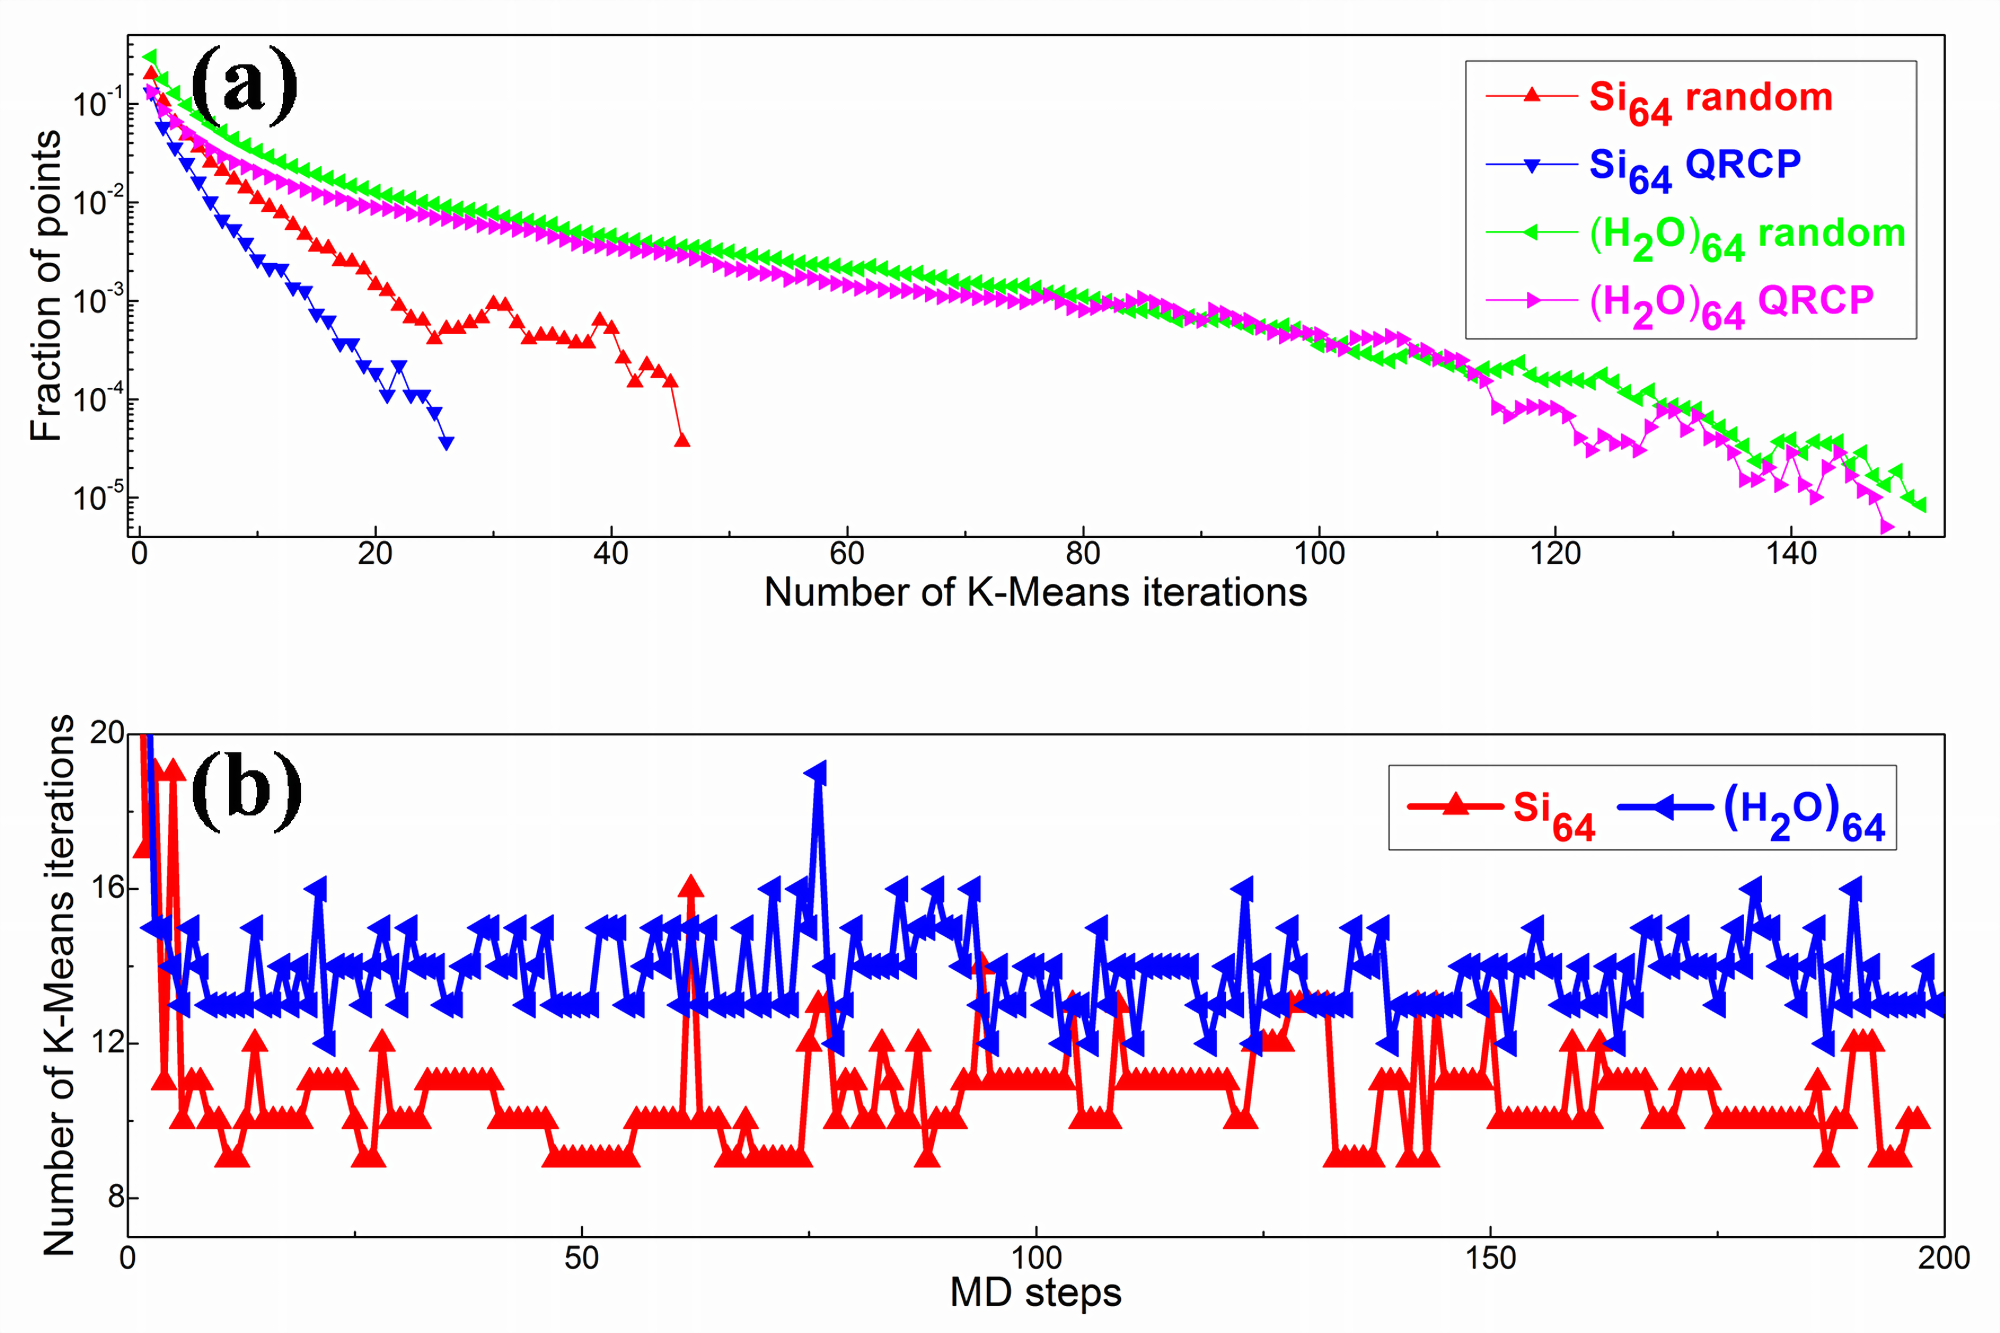
\includegraphics[width=\textwidth]{./cvt/pics/Si64H2O64MD.pdf}
	\end{center}
	\caption{Comparison of the ISDF-CVT method by using either random or
	QRCP initialization for hybrid DFT AIMD simulations on bulk silicon
	system Si$_{64}$ and liquid water system (H$_2$O)$_{64}$, including
	(a) the fraction of points what switch cluster in each K-Means
	iteration and (b) the number of K-Means iterations during each MD
	step.}\label{fig:Si64H2O64MD}
\end{figure}

Figure~\ref{fig:Si64MD} (a) shows that both the CVT-based and QRCP-based ISDF
decomposition lead to controlled energy drift, defined as $E_{\mathrm{drift}}(t)
= (E_{\mathrm{tot}}(t)- E_{\mathrm{tot}}(0))/E_{\mathrm{tot}}(0)$. In the NVE
simulation on bulk silicon system Si$_{64}$, the energy drift per atom is $6.6
\times 10^{-5}$, $7.5 \times 10^{-5}$ and $2.5 \times 10^{-5}\HaPps$
respectively for the ISDF-CVT, ISDF-QRCP, and the conventional nested two-level
SCF iteration procedure, indicating that ISDF is a promising method for
reducing the cost of hybrid functional calculations with controllable loss of
accuracy. Figure~\ref{fig:Si64MD} (b) shows the total potential energy obtained
by the three methods along the MD trajectory, and the difference among the three
methods is more noticeable. This is due to the fact that ISDF decomposition is a
low rank decomposition for the pair product of orbitals, which leads to error in
the Fock exchange energy and hence the total potential energy. Nonetheless, we
find that such difference mainly results in a shift of the potential energy
surface along the MD trajectory, and hence has little affect on physical
observables defined via relative potential energy differences. Furthermore, the
CVT method yields a potential energy trajectory that is much smoother compared
to that obtained from QRCP. This is because the interpolation points obtained
from CVT are driven by the electron density, which varies smoothly along the MD
trajectory. Such properties do not hold for the QRCP method. This means that the
CVT method can be more effective when a smooth potential energy surface is
desirable, such as in the case of geometry optimization. The absolute error of
the potential energy from the CVT method is coincidentally smaller than that
from QRCP, but again we are not aware of any reason for this behavior to hold in
general.

\begin{figure}[htbp]
	\begin{center}
		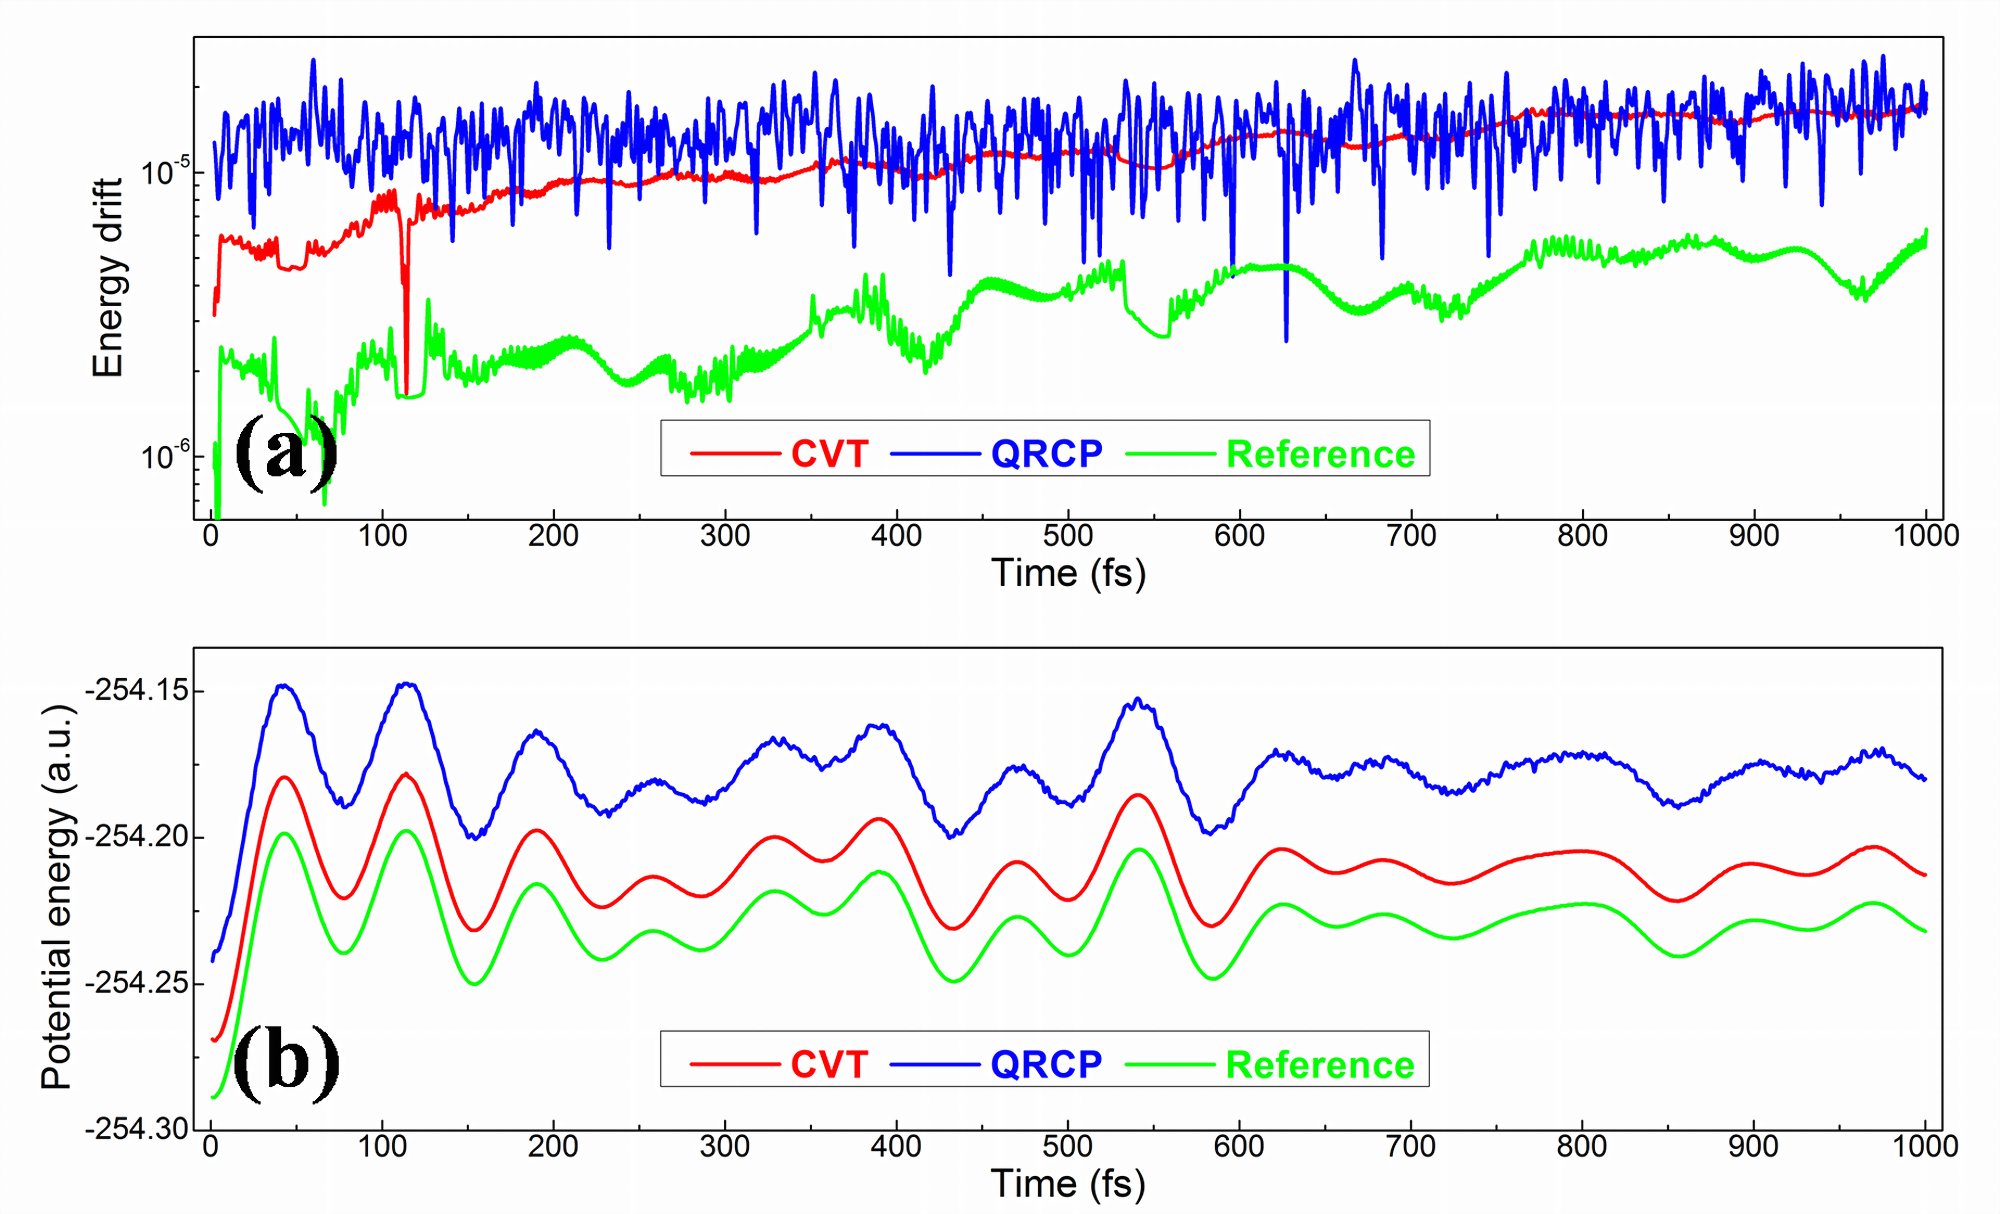
\includegraphics[width=\textwidth]{./cvt/pics/Si64MD.pdf}
	\end{center}
	\caption{Comparison of hybrid HSE06 DFT AIMD simulations by using
	the ISDF-CVT and ISDF-QRCP methods as well as exact nested two-level
	SCF iteration procedure as the reference on the bulk silicon
	Si$_{64}$, including (a) relatively energy drift and (b) potential
	energy during MD steps.} \label{fig:Si64MD}
\end{figure}
\FloatBarrier

We also apply the ACE-ISDF (CVT) and ACE-ISDF (QRCP) methods for hybrid DFT AIMD
simulations on liquid water system (H$_2$O)$_{64}$ under the NVT ensemble to
sample the radial distribution function in Figure~\ref{fig:H2O64gOO}. We find
that the results from all three methods agree very well, and our result is in
quantitative agreement with previous hybrid functional calculations
\cite{JCP_141_084502_2014}, which uses a different exchange-correlation
functional (PBE0) and Van der Waals functional (TS-vdW) 
\cite{PRL_102_073005_2009}.

\begin{figure}[htbp]
	\begin{center}
		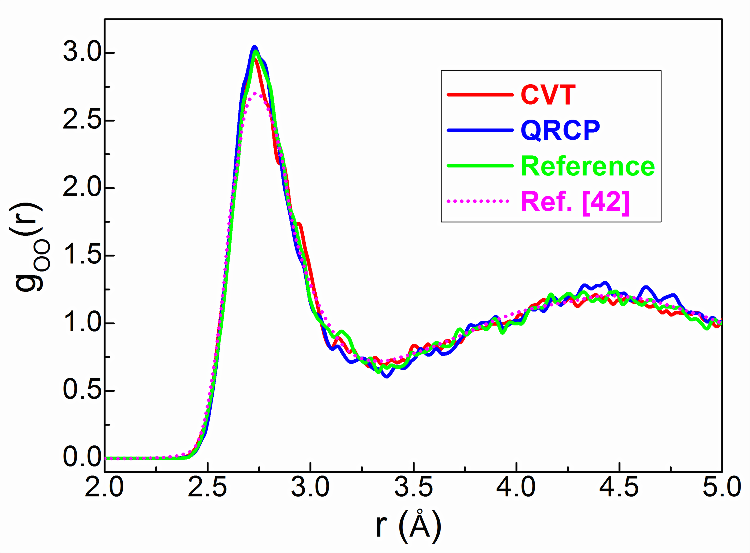
\includegraphics[width=\textwidth]{./cvt/pics/H2O64gOO.pdf}
	\end{center}
	\caption{The oxygen-oxygen radial distribution functions $g_\text{OO}$($r$) of
	liquid water system (H$_2$O)$_{64}$ at $T$ = $295\Kelvin$ obtained from hybrid
	HSE06 + DFT-D2 AIMD simulations with the ISDF-CVT and ISDF-QRCP methods, exact
	nested two-level SCF iteration procedure (as the reference) as well as
	previous hybrid PBE0 + TS-vdW calculation \cite{JCP_141_084502_2014}.}
	\label{fig:H2O64gOO}
\end{figure}
\FloatBarrier
